\documentclass[a4full,12pt]{article}

\title{Integrating a Category-Partition Testing Tool with Combinatorial Interaction
Testing Tool To Produce T-Way Adequate Test Frames}
\author{Andrew Graff}

%\usepackage{fullpage}
%\usepackage{epsfig}
\usepackage{graphicx}
\usepackage{xcolor}
\graphicspath{ {./images/} }
\usepackage{hyperref}
\hypersetup{
    colorlinks=true,
    linkcolor=blue,
    filecolor=magenta,      
    urlcolor=cyan
}
\newcommand{\eas}[1]{{\color{blue}\sf ({#1})}}
\newcommand{\ag}[1]{{\color{red}\sf ({#1})}}
\renewcommand{\topfraction}{.9}
\renewcommand{\bottomfraction}{.9}
\renewcommand{\textfraction}{.1}
\begin{document}
\maketitle
\section{Introduction}
Software is the beating heart of almost every company, which makes defects in that software
 to be potentially very costly. Some software defects result in printing funny characters to the terminal, while others can bring
  company production to a halt for hours or even days, costing thousands and even millions of
  dollars in losses. Another critical defect may result in a security breach, which exposes the company's intellectual property that
  could be fatal to business altogether. That is why testing is such an important part in
  the process of creating defect free software. Testing software is a difficult task, which
  depends on the complexity of the software itself, what kind of inputs it takes, i.e., the input domain, and how
  many functions it performs. Depending on software, testers can choose among different testing approaches
  to implement the actual testing: black-box, white-box, model-based testing, to name a few. In this project, we   
  focus on black-box testing, and more specifically on the test-case optimization: how to generate defect-revealing test cases with a realistically executable number of them.
  
\section{Problem Statement and Proposed Solution}
It is difficult to engineer a set of tests that adequately tests a particular piece of software
  in an acceptable amount of time. Category partitioning is a useful black-box testing method that
  helps systematically design test cases. It allows the user to divide
   the software's input space into categories of choices. \emph{tsl} (testing specification language) is a tool
  that offers a good front-end interface for the category partitioning method with a formal descriptive language
  to specify categories and choices on the input domain partitions. In addition, \emph{tsl} generates readable test frames in an output file, where each test frame corresponds to a test case. However, its weakness is that it generates many frames because it computes all possible permutations of the categories of choices. This results in a large test suite, which may not run in a feasible amount of time.
  
Combinatorial interaction testing (CIT) addresses this problem of the brute force approach of exhaustive test case generation 
by offering a method for analyzing and selecting a subset of test cases
  that cover specific combinations of category choices. The tool we use for CIT is \emph{casa},
  which uses a simulated annealing search to find the subset of test cases with desired interactions between choices. Given a model file and
  constraints file as input, \emph{casa} then outputs to a file with a set of combinations of options, i.e., category choices, that should
  be tested together. The weakness for \emph{casa} is that the constraints are expressed in the conjunctive
  normal form, which is not how a typical user would define or express them. It is much easier and more human
  readable if we could write constraint as a general formula in propositional logic. Thus, it can be challenging for users to write the constraints in \emph{casa}.  Additionally, the output is a set of numbers representing each choice. It's hard to map these numbers back
  to actual choices. So some remapping is required back to the original inputs (e.g. \emph{tsl} ``choices'').
 
These two methodologies and tools are separate pieces of software that require the user to create the input files
  to each tool separately.  {\bf The objective of this project is to combine the user-friendly input/output components
  of \emph{tsl} and integrates them into the powerful test case optimization algorithm of \emph{casa}}. Upon completion of
  the project, we will produce a tool where a user only needs to generate the category partition test specification input file, and an
  easy to use t-test adequate coverage set of test frames will be generated. This will eliminate the necessity for the
  user to generate the complicated and bug prone inputs to the \emph{casa} tool and remapping of the output back into the \emph{tsl} frames.
  
\section{Background}
This project builds on previous work that addresses to
  two different problems: systematic test case generation and test case optimization. In this section we explain approaches for solving each problem and the tools implementing those solutions.

\subsection{Category-partition Method}
The \emph{category-partition method} uses a formal test specification language (TSL) to define
test cases and then generates test case descriptions according to it specification. These test case descriptions are then used to
  create an executable software test suite. As with any formal specification, writing the formal test 
  specifications is an iterative approach. Depending on the size of the software system to test, the 
  engineer may need to break the program up into smaller testable blocks. For 
  the purposes of this project, we will use a simple example of a browser's 
  settings for how to treat tabs. See Figure \ref{fig:tabs_example}.
\begin{figure}[htb]
\centering
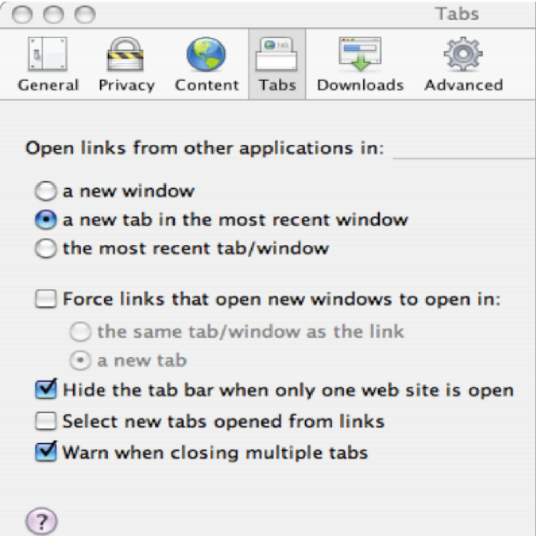
\includegraphics[width=2.3in,keepaspectratio]{images/tabs_example.png}
\caption{Sample of software feature to test tabs}
\label{fig:tabs_example}
\end{figure}

As part of the process to translate this feature into the formal language of \emph{tsl},
  we need to follow a specific format for the test specification file. It specifies
  \emph{categories}, \emph{choices}, \emph{properties}, and \emph{selectors} where 
  \emph{selectors} are boolean expressions. See Figure \ref{fig:tsl_format} for an example.
\begin{figure}[htb]
\centering
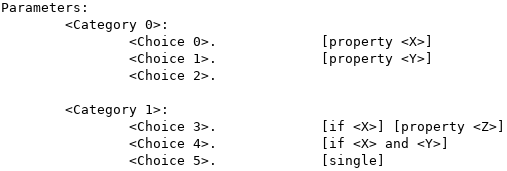
\includegraphics[width=3in,keepaspectratio]{images/tsl_format.png}
\caption{Format for tsl input file}
\label{fig:tsl_format}
\end{figure}

In our example, we need to choose \emph{categories} and \emph{choices} within those
  \emph{categories}. For example, one \emph{category} could be `Link', and the choices
  associated with `Link' are `new window', `new tab', and `current tab' pulled from the
  `Open links from other applications in:' portion of the settings. We complete this step for all
  the available selections in this browser's 'Tabs' options. Next, we assign some 
  \emph{properties}, which are useful for defining constraints that should be imposed on
  the valid \emph{choices} a program may accept. And then the \emph{selectors} are defined
  as prepositional logic statements that select the option that is associated with the 
  \emph{property} that is referenced in the \emph{selector} statement. See Figure \ref{fig:tsl_input_final} for an example.
\begin{figure}[htb]
\centering
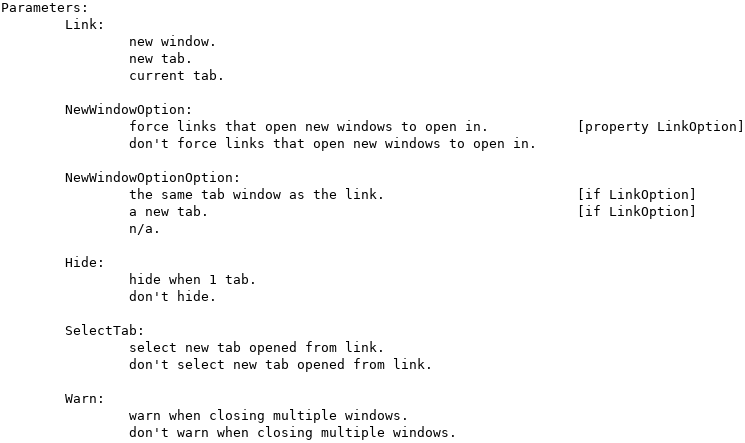
\includegraphics[width=4in,keepaspectratio]{images/tsl_input_final.png}
\caption{An input file for \emph{tsl} using our 'Tabs' example.}
\label{fig:tsl_input_final}
\end{figure}

After \emph{tsl} processes this input file, it produces 96 total test frames
  for all possible combinations of our 'Tabs' example, restricted by the set of constraints. This is a small example with very
  few choices. Another, more complex system such as an airplane cockpit with many switches
  and inputs can produce a large amount of possible combinations, which is not feasible to execute and hence to test this system completely at a certain level of details. Removing categories and or excluding some values might result in smaller but less powerful test suite. Thus, we look for another way to reduce the number of test sets down to a feasible number, yet maintaining the desired level of detail. The original \emph{tsl} tool is written in C and consists of 12 files and 1,125 lines of code.

\subsection{Combinatorial Interaction Testing}
\emph{Combinatorial interaction testing} is a test case selection approach that relies on the principle
  that a large portion of faults can be detected with a smaller subset of test cases that insure interaction
  of different choices for different categories.  \emph{casa} is a tool that finds test cases with a \emph{t-way} covering 
  combinations of choices. The tool uses the simulated annealing search algorithm in order to find
  the minimal set of such test cases.
  
  The tool takes two files as input: one that specifies the \emph{t-way} interaction
  level desired along with all possible inputs and another that encodes constraints on those
  inputs. The output is the subset of combinations that satisfy the selected \emph{t-way}
  interaction level. This allows to identify the subset of tests necessary to get adequate
  t-way testing coverage. In \emph{casa}, the options must be manually written by the user as well as the constraints
  file, which accepts constraints in a conjunctive normal form (CNF). The user can find it difficult to translate from the logical formula of \emph{tsl} to its CNF representation. In addition, the output needs some manipulation to translate it into a readable testing specification.
  
The \emph{casa} tool's \emph{.citmodel} input file has the following format. The first line
  specifies the strength of the T-way pairs to cover, which usually is limited to 2-way or 3-way interaction. The second line specifies the number
  of \emph{categories} we have broken the program into. And the third line specifies how
  many \emph{choices} within each category can be chosen. The enumeration starts from the first \emph{category} to
  the last, e.g., Figure~\ref{fig:casa_citmodel_input}. 
  
  Next, the \emph{.constraints}
  file contains the constraints written as a conjunction of disjunctions, i.e., CNF. The first line
denotes how many disjunctive clauses (constraints) are defined for this model. Each
  conjunctive clause consists of a pair of lines, the first of which specifies how many terms
are in the disjunctive clause. The second line of the pair is the disjunctive clause itself. See Figure \ref{fig:casa_constraints} for a demonstration.

Finally, let us consider the output format from the \emph{casa} program. The first line contains
  the number of combinations generated for the given \emph{.citmodel} and \emph{.constraints}
  input followed by that number of lines, each a different input combination. Each digit in
  the combination represents the \emph{choice} from the \emph{category} in order of their
  defined input. For example, with an input of `2 3 4 5' in our \emph{.citmodel}, the first
  entry of the output line could contain `0' or `1'. The second entry could contain `2', `3',
  or `4'. The third entry would contain `5', `6', `7' or `8', etc. This output could be used
  to generate test frames by associating each entry in the line with its corresponding
  \emph{choice}. See Figure \ref{fig:casa_output}. The \emph{casa} tool consists of 87 files
  with 9,139 lines of code and is written in C++.
  
\begin{figure}[htb]
\centering
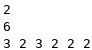
\includegraphics[width=1in,keepaspectratio]{images/casa_citmodel_input.png}
\caption{Example of \emph{casa} .citmodel input file}
\label{fig:casa_citmodel_input}
\end{figure}

\begin{figure}[htb]
\centering
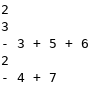
\includegraphics[width=1in,keepaspectratio]{images/casa_constraints.png}
\caption{Constraints file for the `Tabs' example with 2 rules. If option 3 is chosen, then choose 5 or 6. If option 4 is chosen, then choose 7 only.}
\label{fig:casa_constraints}
\end{figure}

\begin{figure}[htb]
\centering
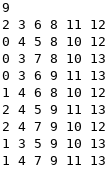
\includegraphics[width=1.25in,keepaspectratio]{images/casa_output.png}
\caption{Output from \emph{casa}}
\label{fig:casa_output}
\end{figure}

\section{Preliminary Work}
Some preliminary work has been done on this project in order to determine the
  feasibility of the idea to combine the \emph{tsl} and \emph{casa} tools into 
  a single, easy to use tool that combines the \emph{tsl}'s front-end and \emph{casa}'s powerful search engine. A goal of the project is to simplify and reduce the
  effort a user needs to put in to use the new tool. Source code was acquired for
  both tools and some initial analysis of the code was done in order to understand
  how they work and where some work may be needed to combine them. As it
  turns out, the \emph{tsl} tool is written in basic C and \emph{casa} is written
  in C++. Converting \emph{tsl} to C++ would be beneficial for combining the 
  code bases into a single program. So \emph{tsl} was updated to support compilation
  with the g++ compiler.

As part of the simplification of the tool, only the category partition test specifications
  should be created by the user as a \emph{.tsl} file. The tool will do the rest to
  generate the adequate coverage set of test frames. Since \emph{casa} takes as input a 
  \emph{.citmodel} file, this preliminary version of \emph{tsl} generates one based on the
  specification file passed in. The support for generation of the \emph{.constraints} file will be added
  at a later time as part of the proposed work. In order to create the \emph{.citmodel}, we need
  to be able to keep track of the parsed information from the specifications file.
  
In order to achieve this, a new struct was added to \texttt{tsl/structs.h} called \texttt{container} that
  keeps track of the list of non-single \texttt{Choices} as a vector of \texttt{Choice} struct
  pointers. This vector is used to look up the choices and categories later for
  printing the test frames. In addition, a \texttt{parent} pointer was added to
  the \texttt{Choice }struct so that the \texttt{Category} information can be referenced when
  performing the lookup into the \texttt{Choice*} vector.
  
Rather than output directly all possible test frames, a new function called
  \texttt{make\_citmodel()} was written in \emph{tsl/output.c} to write a 
  \emph{.citmodel} file used as an input to \emph{casa}. The function
\texttt{generator(Flag flags)} was also modified to call \texttt{make\_citmodel()},
  and then make a system call to casa passing in the \emph{.citmodel} file for
  the input. Then, another function created  called
\texttt{process\_output\_file(string filename)} processes the file output by
  \emph{casa} to generate the test frame final output. Ideally there should be
  no file required, but this is a preliminary draft of the final solution
  and this will be addressed in the final version of the project.
  
  \section{Proposed Remaining Work}
The goal is to simplify the work of a user who needs to use these tools to generate test frames
  for testing. Having a simple user interface and easy to understand input file is key. \emph{tsl}'s
  input format is easy to configure and more user-friendly, so the new tool will inherit this format.
  Our preliminary work has demonstrated feasibility of \emph{tsl} to interact with \emph{casa}.
  
The remaining step is to convert the logic formula from the \emph{properties} and \emph{selectors}
  into CNF accepted by \emph{casa}. One converter in particular, Vojkan Cvijovic's CNF converter is
  available at GitHub (\url{https://github.com/Vojkan-Cvijovic/CNF-Converter/tree/master/src/converter}),
  and it's written in C++ which matches the language for \emph{tsl} and
  \emph{casa}. If this tool does not serve the purpose, another CNF conversion tool will need to be
  found or a new one using well know algorithms for converting a propositional formula into its CNF
  will need to be coded in the \emph{tsl} tool to output the \emph{.constraints} file. The final
  output from the combined tools should be a set of test frames whose number has been reduced in size
  to provide adequate t-way coverage testing of the system described in the input of the program that
  can be quickly actionable from the user to use.
  
My project can be found at the following url \url{https://github.com/Panik-Kontrol/MastersProject}.
  The top-level directory contains my \emph{.tex} files for this proposal as well as a place
  holder for the final paper (not started yet). It will also be the location where I store the
  slides I will present for the proposal next week. The \texttt{src/} directory contains the source
  code for both the \emph{casa} tool and the \emph{tsl} tool that I have and will be modifying.
  The \texttt{images/} directory contains all the figure images used in this proposal.
  
  \subsection{Timeline}
  Here is my tentative timeline
  \begin{itemize}
  \item May, 2021 -- Study Cvijovic's CNF conversion tool and implement converter component.
  \item June, 2021 -- Finish Master's Project description document and defend Master's Project
  \end{itemize}

\end{document}
